% Created 2023-05-11 Thu 19:36
% Intended LaTeX compiler: pdflatex
\documentclass[aspectratio=169,t]{beamer}
\usepackage[utf8]{inputenc}
\usepackage[T1]{fontenc}
\usepackage{graphicx}
\usepackage{longtable}
\usepackage{wrapfig}
\usepackage{rotating}
\usepackage[normalem]{ulem}
\usepackage{amsmath}
\usepackage{amssymb}
\usepackage{capt-of}
\usepackage{hyperref}
\usepackage{listings}
\setbeamerfont{caption}{size=\footnotesize}
\usepackage{animate}
\usepackage{mathtools}
\DeclarePairedDelimiter\abs{\lvert}{\rvert} % ABS: abs{}
\newcommand{\mcb}[2]{\colorbox{#1}{$\displaystyle #2$}}
\usetheme{focus}
\author{Samuel J Monson}
\date{2023-05-16}
\title{Complex and Hypercomplex \\ Iterative Methods}
\institute{Seattle Univerisity}
\definecolor{main}{HTML}{93361f}
\definecolor{background}{HTML}{D0D0D0}
\setmathfont{Fira Math}
\setmathfont{DejaVu Math TeX Gyre}[range=\vysmwhtcircle]
\setmonofont{Hack}
\hypersetup{
 pdfauthor={Samuel J Monson},
 pdftitle={Complex and Hypercomplex \\ Iterative Methods},
 pdfkeywords={},
 pdfsubject={},
 pdfcreator={Emacs 30.0.50 (Org mode 9.6.1)}, 
 pdflang={English}}
\begin{document}

\begin{frame}
\maketitle
\end{frame}
\section{Introduction}
\label{sec:org6c7cd28}

\begin{frame}[label={sec:org9b4ceb0}]{Iteration}
\begin{definition}[Function Iteration]\label{sec:org73f8cbb}
\(f^0 := \symbf{I}\)

\(f^{k+1} := f \circ f^k\)
\end{definition}

\begin{exampleblock}<2->{Example}\label{sec:org63bde76}
Given \(f(x) = x + 1\),

\begin{align*}
    \onslide<3->{f^0(x) & = x \\}
    \onslide<4->{f^1(x) & = x + 1 \\}
    \onslide<5->{f^2(x) & = (x + 1) + 1 \\}
    \onslide<6->{f^3(x) & = \left((x + 1) + 1\right) + 1}
\end{align*}
\end{exampleblock}
\end{frame}

\begin{frame}[label={sec:orgb6383fd}]{Complex Dynamics}
\begin{definition}[Dynamical System]\label{sec:org1e8bfce}
A system that enacts rules on a set of variables to produce a state.
\end{definition}

\begin{definition}<2->[Complex Dynamics]\label{sec:org2f84c24}
The study of \uline{dynamical systems} defined by complex functions.
\end{definition}
\end{frame}


\begin{frame}[label={sec:org6b34434}]{Complex Numbers}
\begin{definition}[Complex Numbers]\label{sec:orgfefaf5a}
\(\symbf{i}^2 = -1\)

\(\{a + b \symbf{i} : a,b \in \symbb{R} \} \in \symbb{C}\)
\end{definition}

\begin{columns}
\begin{column}{0.5\columnwidth}
\begin{block}<2->{Addition}
\begin{itemize}
\item<2-> Let \(a,b,x,y \in \symbb{R}\),
\end{itemize}
\begin{align*}
    \onslide<3->{(a + b\symbf{i}) + (x + y\symbf{i})} \onslide<4->{& = (a + x) + (b + y)\symbf{i}}
\end{align*}
\end{block}
\end{column}

\begin{column}{0.5\columnwidth}
\begin{block}<5->{Multiplication}
\begin{itemize}
\item<5-> Let \(a,b,x,y \in \symbb{R}\),
\end{itemize}
\begin{align*}
    \onslide<6->{(a + b\symbf{i}) \times (x + y\symbf{i})} \onslide<7->{& = ax + ay\symbf{i} + bx\symbf{i} + by\symbf{i}^2 \\}
    \onslide<8->{& = (ax - by) + (ay + bx)\symbf{i}}
\end{align*}
\end{block}
\end{column}
\end{columns}
\end{frame}

\section{Complex Iterative Methods}
\label{sec:org7a82696}

\begin{frame}[label={sec:orgc355175}]{Complex Iteration}
\begin{columns}
\begin{column}{0.5\columnwidth}
\begin{block}{Rules}
\(f(z) = z^2\)

\(z_0 = \frac{1}{\sqrt{2}} + \frac{1}{\sqrt{2}} \symbf{i}\)
\end{block}

\begin{itemize}[<+->]
\item \(f^0(z) = \frac{1}{\sqrt{2}} + \frac{1}{\sqrt{2}} \symbf{i}\)
\item \(f^1(z) \only<2>{= \left( \frac{1}{\sqrt{2}} + \frac{1}{\sqrt{2}} \symbf{i} \right)^2 = \left( \frac{1}{\sqrt{2}} \right)^2 - \left(\frac{1}{\sqrt{2}} + \frac{1}{\sqrt{2}}\right)^2 + \left(\frac{1}{\sqrt{2}} + \frac{1}{\sqrt{2}}\right)^2 \symbf{i}} = \symbf{i}\)
\item \(f^2(z) = -1\)
\item \(f^3(z) = 1\)
\item \(f^4(z) = f^5(z) = f^6(z) = 1\)
\end{itemize}
\end{column}

\begin{column}{0.5\columnwidth}
\begin{center}
\includegraphics<1>[width=.9\linewidth]{Figs/exports/Iter_1-0.png}
\includegraphics<2>[width=.9\linewidth]{Figs/exports/Iter_1-1.png}
\includegraphics<3>[width=.9\linewidth]{Figs/exports/Iter_1-2.png}
\includegraphics<4->[width=.9\linewidth]{Figs/exports/Iter_1-3.png}
\end{center}
\end{column}
\end{columns}
\end{frame}

\begin{frame}[label={sec:org3a0ce9a}]{Complex Iteration}
\begin{columns}
\begin{column}{0.5\columnwidth}
\begin{block}{Rules}
\(f(z) = z^2 - \frac{1}{10} - \frac{1}{10} \symbf{i}\)

\(z_0 = \frac{1}{\sqrt{2}} + \frac{1}{\sqrt{2}} \symbf{i}\)
\end{block}

\begin{itemize}[<+->]
\item \(f^0(z) = \frac{1}{\sqrt{2}} + \frac{1}{\sqrt{2}} \symbf{i}\)
\item \(f^1(z) \only<2>{= -\frac{1}{10} + \left(1 - \frac{1}{10}\right)\symbf{i}} = -0.1 + 0.9\symbf{i}\)
\item \(f^2(z) = -0.9-0.28\symbf{i}\)
\item \(f^3(z) = 0.6316+0.404\symbf{i}\)
\item \(f^4(z) \approx 0.13570256+0.4103328\symbf{i}\)
\item \(f^5(z) \approx -0.24995782+0.01136642\symbf{i}\)
\item \(f^6(z) \approx -0.03765028-0.10568225\symbf{i}\)
\end{itemize}
\end{column}

\begin{column}{0.5\columnwidth}
\begin{center}
\includegraphics<1>[width=.9\linewidth]{Figs/exports/Iter_2-0.png}
\includegraphics<2>[width=.9\linewidth]{Figs/exports/Iter_2-1.png}
\includegraphics<3>[width=.9\linewidth]{Figs/exports/Iter_2-2.png}
\includegraphics<4>[width=.9\linewidth]{Figs/exports/Iter_2-3.png}
\includegraphics<5>[width=.9\linewidth]{Figs/exports/Iter_2-4.png}
\includegraphics<6>[width=.9\linewidth]{Figs/exports/Iter_2-5.png}
\includegraphics<7->[width=.9\linewidth]{Figs/exports/Iter_2-6.png}
\end{center}
\end{column}
\end{columns}
\end{frame}

\begin{frame}[label={sec:org137cee5}]{Group Activity}
\(f(z) = z^2 + c\)

\begin{columns}
\begin{column}{0.5\columnwidth}
\begin{block}{Easier}
\(c = -0.2 + 0 \symbf{i}\)

\(z_0 = 0.5 + 0 \symbf{i}\)
\end{block}
\end{column}

\begin{column}{0.5\columnwidth}
\begin{block}{Harder}
\(c = -0.2 + 0.4 \symbf{i}\)

\(z_0 = 0.5 - 0.5 \symbf{i}\)
\end{block}
\end{column}
\end{columns}
\end{frame}

\begin{frame}[label={sec:org1937aea}]{Group Activity (Easier)}
\begin{columns}
\begin{column}{0.5\columnwidth}
\begin{block}{Rules}
\(f(z) = z^2 + c\)

\(c = -0.2 + 0 \symbf{i}\)

\(z_0 = 0.5 + 0 \symbf{i}\)
\end{block}

\begin{itemize}[<+->]
\item \(f^0(z) = 0.5\)
\item \(f^1(z) = 0.05\)
\item \(f^2(z) = -0.1975\)
\item \(f^3(z) = -0.16099375\)
\item \(f^4(z) \approx -0.1740810125\)
\end{itemize}
\end{column}

\begin{column}{0.5\columnwidth}
\begin{center}
\includegraphics<1>[width=.9\linewidth]{Figs/exports/Iter_3-0.png}
\includegraphics<2>[width=.9\linewidth]{Figs/exports/Iter_3-1.png}
\includegraphics<3>[width=.9\linewidth]{Figs/exports/Iter_3-2.png}
\includegraphics<4>[width=.9\linewidth]{Figs/exports/Iter_3-3.png}
\includegraphics<5->[width=.9\linewidth]{Figs/exports/Iter_3-4.png}
\end{center}
\end{column}
\end{columns}
\end{frame}

\begin{frame}[label={sec:orgb0391f2}]{Group Activity (Harder)}
\begin{columns}
\begin{column}{0.5\columnwidth}
\begin{block}{Rules}
\(f(z) = z^2 + c\)

\(c = -0.2 + 0.4 \symbf{i}\)

\(z_0 = 0.5 - 0.5 \symbf{i}\)
\end{block}

\begin{itemize}[<+->]
\item \(f^0(z) = 0.5 - 0.5 \symbf{i}\)
\item \(f^1(z) = -0.2 - 0.1 \symbf{i}\)
\item \(f^2(z) = -0.17 + 0.44 \symbf{i}\)
\item \(f^3(z) = -0.3647 + 0.2504 \symbf{i}\)
\item \(f^4(z) = -0.12969407 + 0.21735824 \symbf{i}\)
\end{itemize}
\end{column}

\begin{column}{0.5\columnwidth}
\begin{center}
\includegraphics<1>[width=.9\linewidth]{Figs/exports/Iter_4-0.png}
\includegraphics<2>[width=.9\linewidth]{Figs/exports/Iter_4-1.png}
\includegraphics<3>[width=.9\linewidth]{Figs/exports/Iter_4-2.png}
\includegraphics<4>[width=.9\linewidth]{Figs/exports/Iter_4-3.png}
\includegraphics<5->[width=.9\linewidth]{Figs/exports/Iter_4-4.png}
\end{center}
\end{column}
\end{columns}
\end{frame}

\begin{frame}[label={sec:org62675ac},fragile]{Implementation}
 \begin{columns}
\begin{column}{0.50\columnwidth}
\begin{block}{Iteration (Python)}
\begin{lstlisting}[language=Python,firstnumber=1,numbers=left]
N = 128
B = 16
c = complex(-0.2, 0.4)
def iterate(z):
    for n in range(N):
        z = z*z + c
        if abs(z) > B: break
    return n
\end{lstlisting}
\end{block}
\end{column}

\begin{column}{0.45\columnwidth}
\begin{center}
\includegraphics<2->[width=.9\linewidth]{Figs/exports/Iter_4-128.png}
\end{center}
\end{column}
\end{columns}
\end{frame}

\begin{frame}[label={sec:org13284c0}]{Iterative Fractals}
\begin{columns}
\begin{column}{0.55\columnwidth}
\begin{block}{Complex Juila Set Example}
Defined by iterative function in complex space

\begin{itemize}
\item \(f_c (z) = z^2 + c\)

\item \(\left\{ z_0 \in \symbb{C}: \abs{f^k_c \left(z_0 \right)} \in \symbb{C} \text{ as } k \to \infty\right\} \in K_c\)
\end{itemize}
\end{block}
\end{column}

\begin{column}{0.45\columnwidth}
\begin{figure}[htbp]
\centering
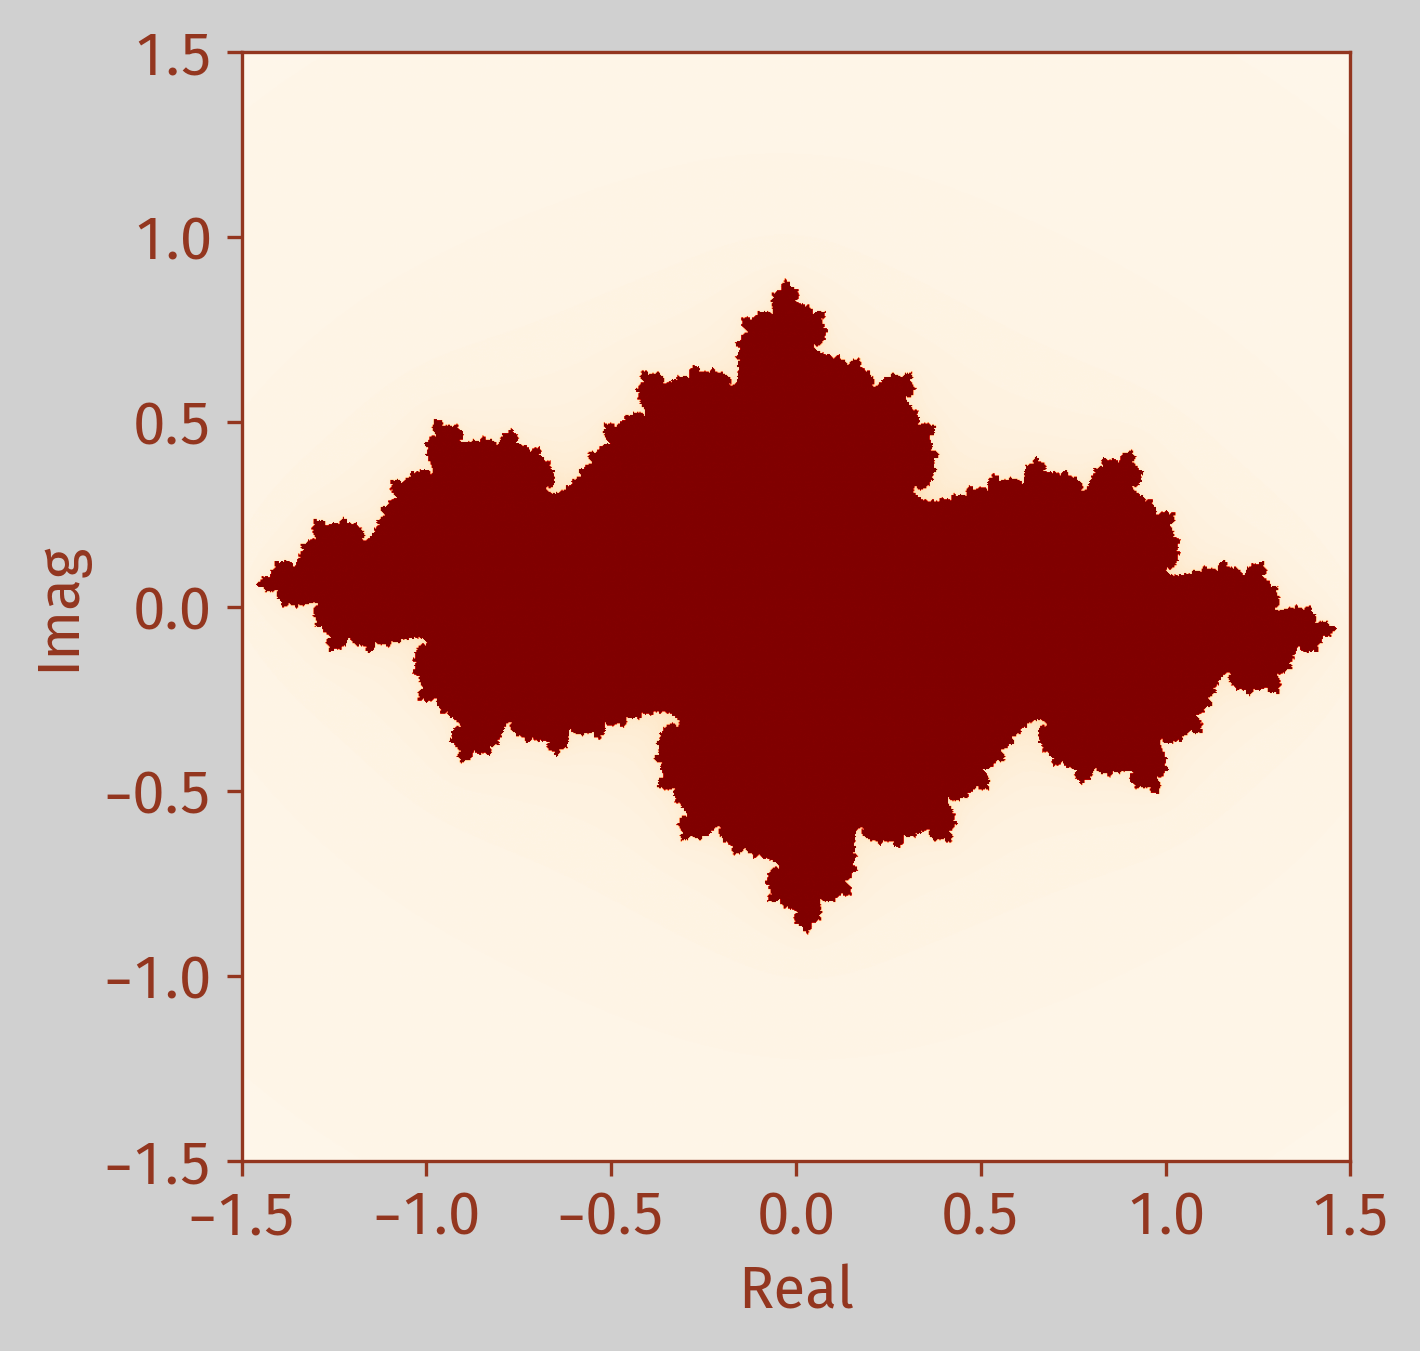
\includegraphics[width=0.80\textwidth]{./Figs/Fig_2v2.png}
\caption{\(f(z) = z^2 -0.675 - 0.112\symbf{i}\)}
\end{figure}
\end{column}
\end{columns}
\end{frame}

\section{Hypercomplex Numbers}
\label{sec:orgf4b76ec}

\begin{frame}[label={sec:orga49fadc}]{Quaternions}
\end{frame}

\begin{frame}[label={sec:org7254f52}]{Quaternions}
\begin{definition}[Quaternion]\label{sec:orga9d9bdf}
\(\symbf{i}^2 = \symbf{j}^2 = \symbf{k}^2 = \symbf{ijk} = -1\)

\(\left\{ d + a\symbf{i} + b\symbf{j} + c\symbf{k} : a,b,c,d \in \symbb{R} \right\} \in \symbb{H}\)
\end{definition}

\begin{columns}
\begin{column}{0.50\columnwidth}
\begin{itemize}
\item<2-> \(\symbf{i}^2 = \symbf{ijk}\)

{\centering
$ \displaystyle
\begin{aligned}
  \symbf{i}^{-1} \symbf{i}^2 & = \symbf{i}^{-1} \symbf{ijk} \\
  \symbf{i} & = \symbf{jk}
\end{aligned}
$
\par}
\item<3-> \(\symbf{k}^2 = \symbf{ijk}\)

{\centering
$ \displaystyle
\begin{aligned}
  \symbf{k}^2 \symbf{k}^{-1} & = \symbf{ijk} \symbf{k}^{-1} \\
  \symbf{k} & = \symbf{ij}
\end{aligned}
$
\par}
\item<3-> \(\symbf{j} = \symbf{ki}\)
\end{itemize}
\end{column}

\begin{column}{0.50\columnwidth}
\begin{itemize}
\item<4-> \(\symbf{i} = \symbf{jk}\)

{\centering
$ \displaystyle
\begin{aligned}
  \symbf{ji} & = \symbf{jjk} \\
  \symbf{ji} & = \symbf{j}^2 \symbf{k} \\
  \symbf{ji} & = -\symbf{k} \\
  -\symbf{k} & = \symbf{ji}
\end{aligned}
$
\par}
\item<5-> \(-\symbf{i} = \symbf{kj}\)
\item<5-> \(-\symbf{j} = \symbf{ik}\)
\end{itemize}
\end{column}
\end{columns}
\end{frame}

\begin{frame}[label={sec:org1117fc6}]{}
\begin{block}{Let,}
\(\symbf{i}^2 = \symbf{j}^2 = \symbf{k}^2 = \symbf{ijk} = -1\)

\(p = d + a\symbf{i} + b\symbf{j} + c\symbf{k}\)

\(q = w + x\symbf{i} + y\symbf{j} + z\symbf{k}\)
\end{block}

\begin{align*}
    p \times q \only<1-2>{& = dw + dx\symbf{i} + dy\symbf{j} + dz\symbf{k} \\}
    \only<1-2>{& + aw\symbf{i} + ax\symbf{i}^2 + ay\symbf{ij} + az\symbf{ik} \\}
    \only<1-2>{& + bw\symbf{j} + bx\symbf{ji} + by\symbf{j}^2 + bz\symbf{jk} \\}
    \only<1-2>{& + cw\symbf{k} + cx\symbf{ki} + cy\symbf{kj} + cz\symbf{k}^2 \\}
    \only<2-3>{& = dw - ax - by - cz\only<4->{+} \\}
    \only<2-3>{& + dx\symbf{i} + aw\symbf{i} + bz\symbf{i} - cy\symbf{i} \\}
    \only<2-3>{& + dy\symbf{j} - az\symbf{j} + bw\symbf{j} + cx\symbf{j} \\}
    \only<2-3>{& + dz\symbf{k} + ay\symbf{k} - bx\symbf{k} + cw\symbf{k} \\}
    \onslide<4->{& = dw - \left\langle\begin{smallmatrix} a\\b\\c \end{smallmatrix}\right\rangle \cdot \left\langle\begin{smallmatrix} x\\y\\z \end{smallmatrix}\right\rangle \\}
    \onslide<4->{& + \left\langle\begin{matrix}}
    \onslide<4->{dx + aw + bz - cy \\}
    \onslide<4->{dy - az + bw + cx \\}
    \onslide<4->{dz + ay - bx + cw}
    \onslide<4->{\end{matrix}\right\rangle}
    \onslide<4->{\cdot \left\langle\begin{matrix} \symbf{i} \\ \symbf{j} \\ \symbf{k} \end{matrix}\right\rangle \\}
    \onslide<5->{& = dw - \left\langle\begin{smallmatrix} a\\b\\c \end{smallmatrix}\right\rangle \cdot \left\langle\begin{smallmatrix} x\\y\\z \end{smallmatrix}\right\rangle + \left(d \left\langle\begin{smallmatrix} x\\y\\z \end{smallmatrix}\right\rangle + w \left\langle\begin{smallmatrix} a\\b\\c \end{smallmatrix}\right\rangle + \left\langle\begin{smallmatrix} a\\b\\c \end{smallmatrix}\right\rangle \times \left\langle\begin{smallmatrix} x\\y\\z \end{smallmatrix}\right\rangle \right) \cdot \left\langle\begin{smallmatrix} \symbf{i}\\\symbf{j}\\\symbf{k} \end{smallmatrix}\right\rangle}
\end{align*}
\end{frame}

\begin{frame}[label={sec:org579cebb}]{Iteration}
\begin{center}
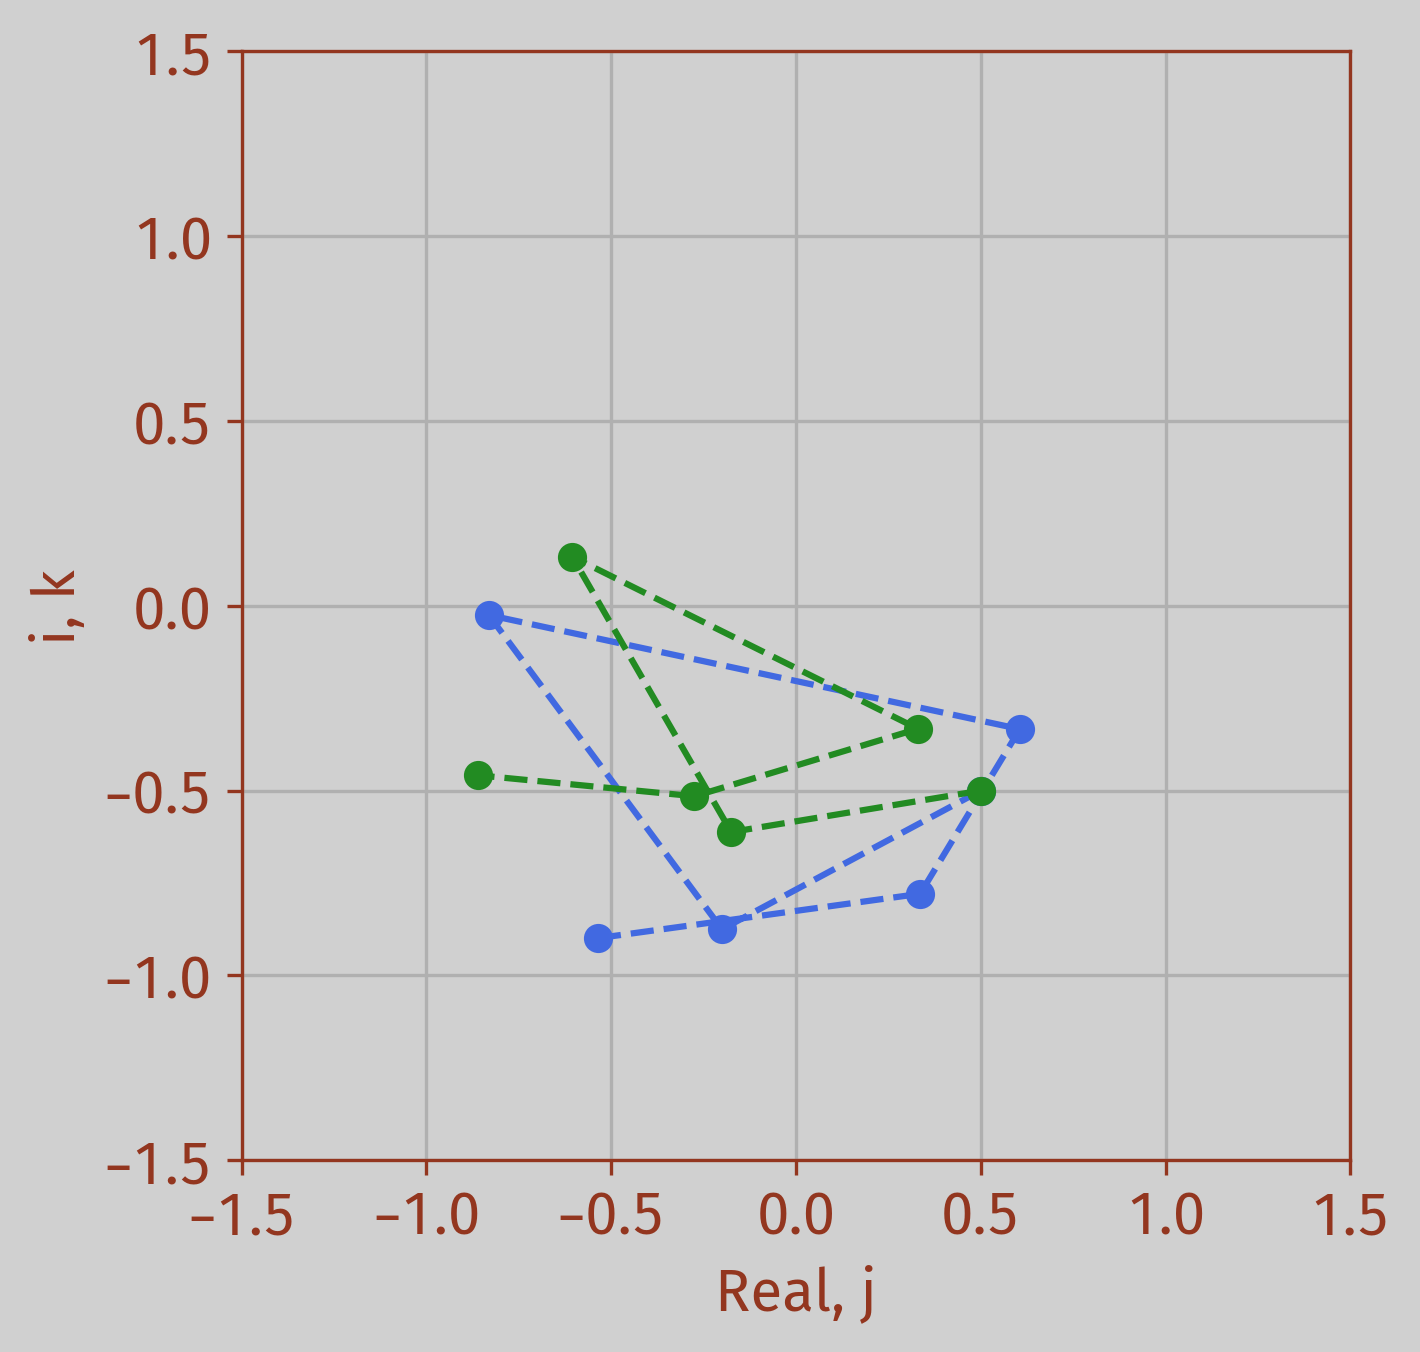
\includegraphics[height=0.70\textheight]{Figs/exports/Iter_5.png}
\end{center}
\end{frame}

\section{Hypercomplex Iterative Methods}
\label{sec:org8116adb}

\begin{frame}[label={sec:org24ad9e4},fragile]{Implementation}
 \begin{block}{Quaternion Multiplication}
\begin{lstlisting}[language=Python,firstnumber=1,numbers=left]
def qMult(p, q):
    r = Quat(
        p.r*q.r – p.i*q.i – p.j*q.j - p.k*q.k,
        p.r*q.i + p.i*q.r + p.j*q.k - p.k*q.j,
        p.r*q.j – p.i*q.k + p.j*q.r + p.j*q.i,
        p.r*q.k + p.i*q.j – p.j*q.i + p.k*q.r
    )
    return r
\end{lstlisting}
\end{block}
\end{frame}

\begin{frame}[label={sec:org5c6721f},fragile]{Implementation}
 \begin{block}{Quaternion Square}
\begin{lstlisting}[language=Python,firstnumber=1,numbers=left]
def qSquare(q):
    r = Quat(
        q.r*q.r – q.i*q.i – q.j*q.j - q.k*q.k,
        2*q.r*q.i,
        2*q.r*q.j,
        2*q.r*q.k
    )
    return r
\end{lstlisting}
\end{block}
\end{frame}

\begin{frame}[label={sec:orgc9cf3e2},fragile]{Implementation}
 \begin{block}{Quaternion Add}
\begin{lstlisting}[language=Python,firstnumber=1,numbers=left]
def qAdd(p, q):
    r = Quat(
        p.r + q.r,
        p.i + q.i,
        p.j + q.j,
        p.k + q.k
    )
    return r
\end{lstlisting}
\end{block}
\end{frame}

\begin{frame}[label={sec:org3cb6bbd},fragile]{Implementation}
 \begin{block}{Iteration}
\begin{lstlisting}[language=Python,firstnumber=1,numbers=left]
N = 12
B = 16
c = Quat(-0.2, 0.4, -0.4, -0.4)
def iterate(z):
    for n in range(N):
        z = z*z + c
        if abs(z) > B: break
    return n
\end{lstlisting}
\end{block}
\end{frame}

\begin{frame}[label={sec:org6b96eff}]{Ploting}
\end{frame}

\begin{frame}[label={sec:orga817103}]{Raytracing}
\end{frame}

\begin{frame}[label={sec:org8b95f81}]{Ray Marching}
\end{frame}

\begin{frame}[label={sec:orgb721ea0}]{Normal Estimation}
\end{frame}

\begin{frame}[label={sec:orga4d6b64}]{Hypercomplex Iterative Fractals}
\begin{columns}
\begin{column}{0.55\columnwidth}
\begin{block}{Hypercomplex Juila Set Example}
\begin{itemize}
\item Defined by iterative function in 4D Quaternion space
\end{itemize}
\end{block}
\end{column}

\begin{column}{0.45\columnwidth}
\begin{figure}[htbp]
\centering
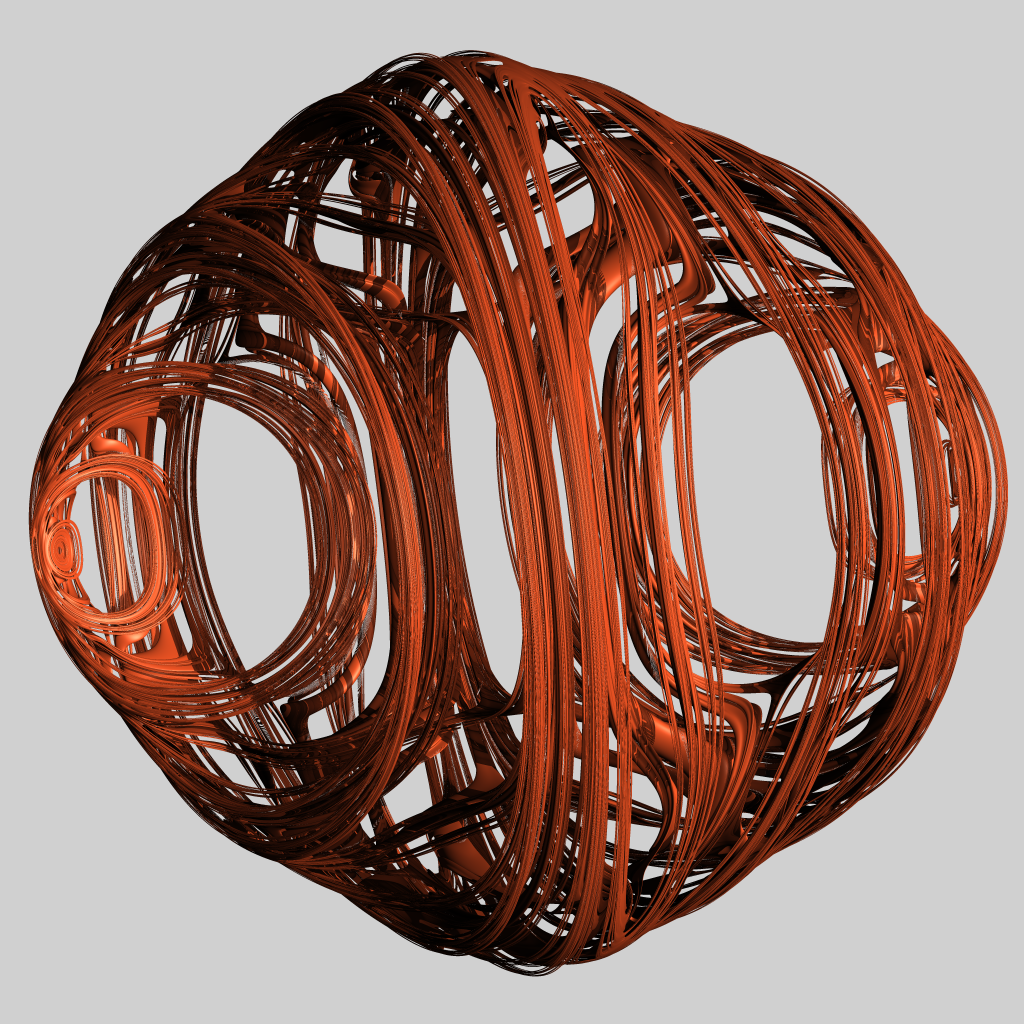
\includegraphics[width=0.75\textwidth]{./Figs/Fig_1v2.png}
\caption{\(f(z) = z^2 + 0.3 - 0.375\symbf{i} - 0.675\symbf{j} - 0.112\symbf{k}\)}
\end{figure}
\end{column}
\end{columns}
\end{frame}

\begin{frame}[label={sec:org4bdb8a3}]{Conclusion}
%\animategraphics[autoplay,interpolate,height=4.0cm,loop]{7}{Figs/Test/}{1}{14}
\setcounter{tocdepth}{2}
\tableofcontents
\end{frame}

\begin{frame}[allowframebreaks,label=]{References}
\nocite{*}
\bibliography{sources}
\bibliographystyle{alpha}
\end{frame}

\begin{frame}[label={sec:orge418bfa}]{Questions?}
\begin{center}
\url{https://github.com/scrufulufugus/senior-synthesis}


\includegraphics[height=0.70\textheight]{./Figs/qr.png}
\end{center}
\end{frame}
\end{document}